\documentclass[10pt,letterpaper,onecolumn]{article}
\usepackage{amsmath}
\usepackage{graphicx} 
\usepackage{hyperref}
\usepackage{xcolor}
\usepackage{subfig}
\graphicspath{ {img/} }
\begin{document}
\bibliographystyle{unsrt}
\title{Measuring the Lifetime of a Muon via Double Scintillator Detection}


\author{
 Akhil Deshpande \\*
 Nirmal Patel \\*
 \\*
 PHY 474 Advanced Laboratory \\*
 Spring 2024 \\*
 Dr. Deepa Thomas \\*
 Department of Physics \\*
 The University of Texas at Austin \\*
 Austin, TX 78712, USA\\
}
\date{\today}
\maketitle

\begin{abstract}
    This experiment utilizes a number of photomultiplier tubes and plastic scintillators to measure the lifetime of muons, elementary particles generated by cosmic rays interacting with Earth's atmosphere. To collect data, we set up a lead glass box, as well as scintillators and photomultiplier tubes to detect when a muon enters the setup. Using a series of signal coincidence detectors, we were able to determine start and stop signals for muons entering the setup and decaying, resulting in a determined 2.43 $\pm$ .22 microseconds for the mean lifetime of the particle.
\end{abstract}
\section{Introduction}
\subsection{Historical Context}
The discovery of the muon in the 20th century marked a pivotal moment in the development of particle physics. Initially observed in cosmic ray experiments by Carl D. Anderson and Seth Neddermeyer at the California Institute of Technology in 1936, the muon ($\mu$) was first mistaken for Yukawa's predicted particle responsible for the nuclear force \cite{StreetStevenson:1937}. Yukawa's meson, theorized in 1935, was expected to mediate the strong interactions within the atomic nucleus, possessing a mass between that of the electron and the proton. However, the properties of the muon, once further analyzed, did not conform to those anticipated for the mediator of the nuclear force. \cite{Yukawa1935}


The muon is a lepton, a class of elementary particles not subject to the strong nuclear force, with a negative electric charge and a mass approximately 207 times that of the electron. \cite{CODATA2018MuonElectronMassRatio} The existence of the muon necessitated a significant expansion of the particle zoo, heralding the beginning of an era that would eventually lead to the establishment of the Standard Model of particle physics.


The clarification of the muon's nature and its differentiation from Yukawa's meson, later identified as the pion ($\pi$), was instrumental in the advancement of quantum field theories. This distinction emphasized the need for a comprehensive framework to understand the plethora of particles being discovered. The subsequent development of quantum electrodynamics (QED) and the electroweak theory, which unified the electromagnetic and weak forces, were partially motivated by the necessity to incorporate the muon and other leptons in a coherent theoretical structure. \cite{MuonG2Experiment2004}
\subsection{Theoretical Background}

The muon ($\mu$) is an elementary particle in the lepton family, akin to the electron but with a significantly greater mass. It carries a charge of $-1e$ and has a spin of $\frac{1}{2}$, classifying it as a fermion under the Standard Model of particle physics. The muon's mass is approximately $105.7 \, \text{MeV}/c^2$, making it about 207 times more massive than the electron. Despite its greater mass, the muon decays to an electron, a neutrino, and an antineutrino, due to the weak interaction, showcasing its unstable nature.

\subsubsection{Muon Decay}

The primary decay mode of the muon is represented by the following equation:
\[
\mu^- \rightarrow e^- + \bar{\nu}_e + \nu_\mu
\]
This decay process is mediated by the weak force, specifically through the exchange of a $W^-$ boson in the virtual state. The Feynman diagram for this decay illustrates the muon decaying into a muon neutrino and a virtual $W^-$ boson, which then converts into an electron and an electron antineutrino. The half-life of the muon in its rest frame is approximately $2.2 \, \mu\text{s}$, a duration that, while brief, allows for extensive experimental study of its decay processes and the verification of the Standard Model predictions. \cite{Beringer2012Leptons}

\subsubsection{Cherenkov Radiation}

When a muon travels through a medium at a speed greater than the phase velocity of light in that medium, it emits Cherenkov radiation, a phenomenon analogous to a sonic boom but with electromagnetic waves. The radiation is emitted at a characteristic angle $\theta$ relative to the direction of the particle's motion, which can be described by the formula:
\[
\cos\theta = \frac{1}{n\beta}
\]
where $n$ is the refractive index of the medium and $\beta$ is the speed of the particle relative to the speed of light in vacuum. 
\cite{Jackson1999Electrodynamics}

\section{Experimental Procedure}
\subsection{Apparatus}
\subsubsection{Overview}
This experiment focuses on detecting the presence of muons through the use of scinillators and photmultiplier tubes. We first set up a plastic scintillator on top of a lead glass box. This top scintillator will detect when a muon first passes through it. Then, the lead glass box (in tandem with a scintillating liquid) will capture the muon, slowing it to rest. The muon will then decay, as shown above. The decay components will be measured by either a left of a right photomultiplier tube (PMT). When these PMTs activate, these signals are timed by our ORTEC setup, and we can achieve a spectrum of the lifetimes of the captured particles. 

An alternate setup we can consider is in the case of a single PMT and scintillator setup. We can wire this setup to a time-to-amplitude (TAC)converter directly. When the muon enters the scintillator, it will activate the PMT, and when it decays, it will again activate the PMT. This difference in times is measured by the TAC, and sorted into 'bins' by a multi-channel analyzer (MCA), such that it again provides us with an exponential decay spectrum.
\begin{figure}
    \begin{center}
        \subfloat[\centering MCA, TAC, and time calibrator]{{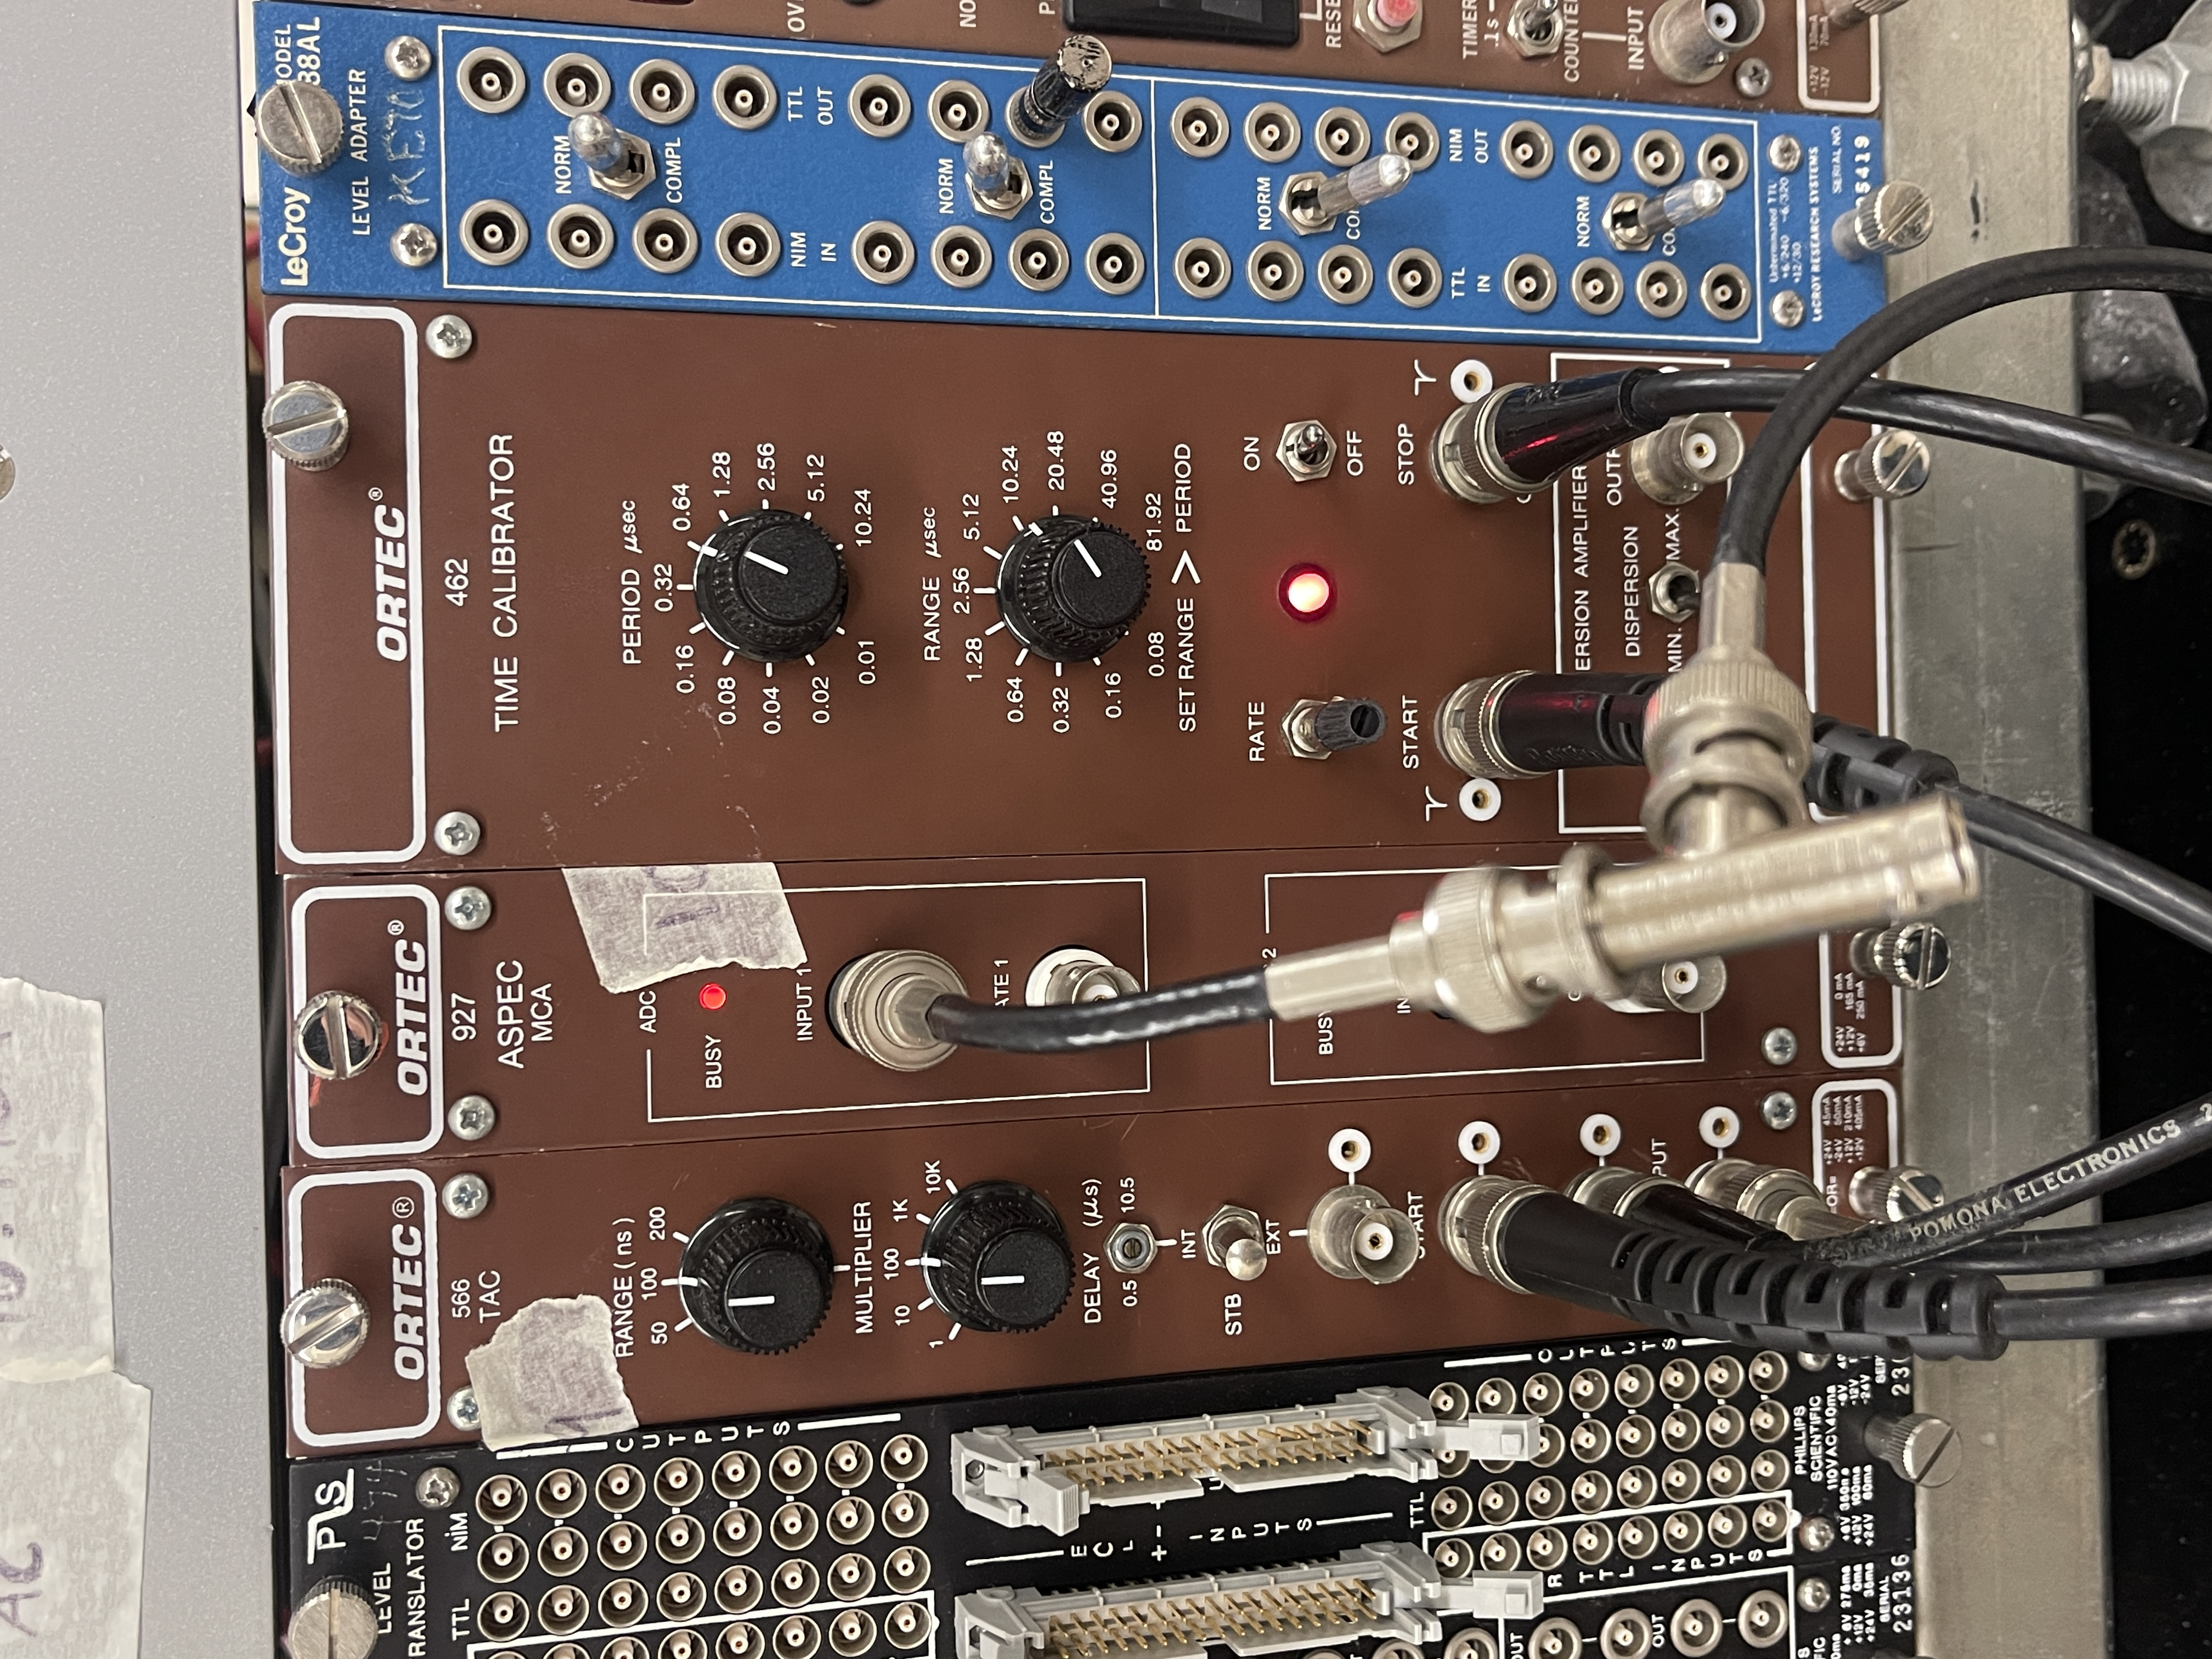
\includegraphics[width=6cm, angle = 270]{Apparatus009.JPG}}}%
        \qquad
        \subfloat[\centering Philips Components]{{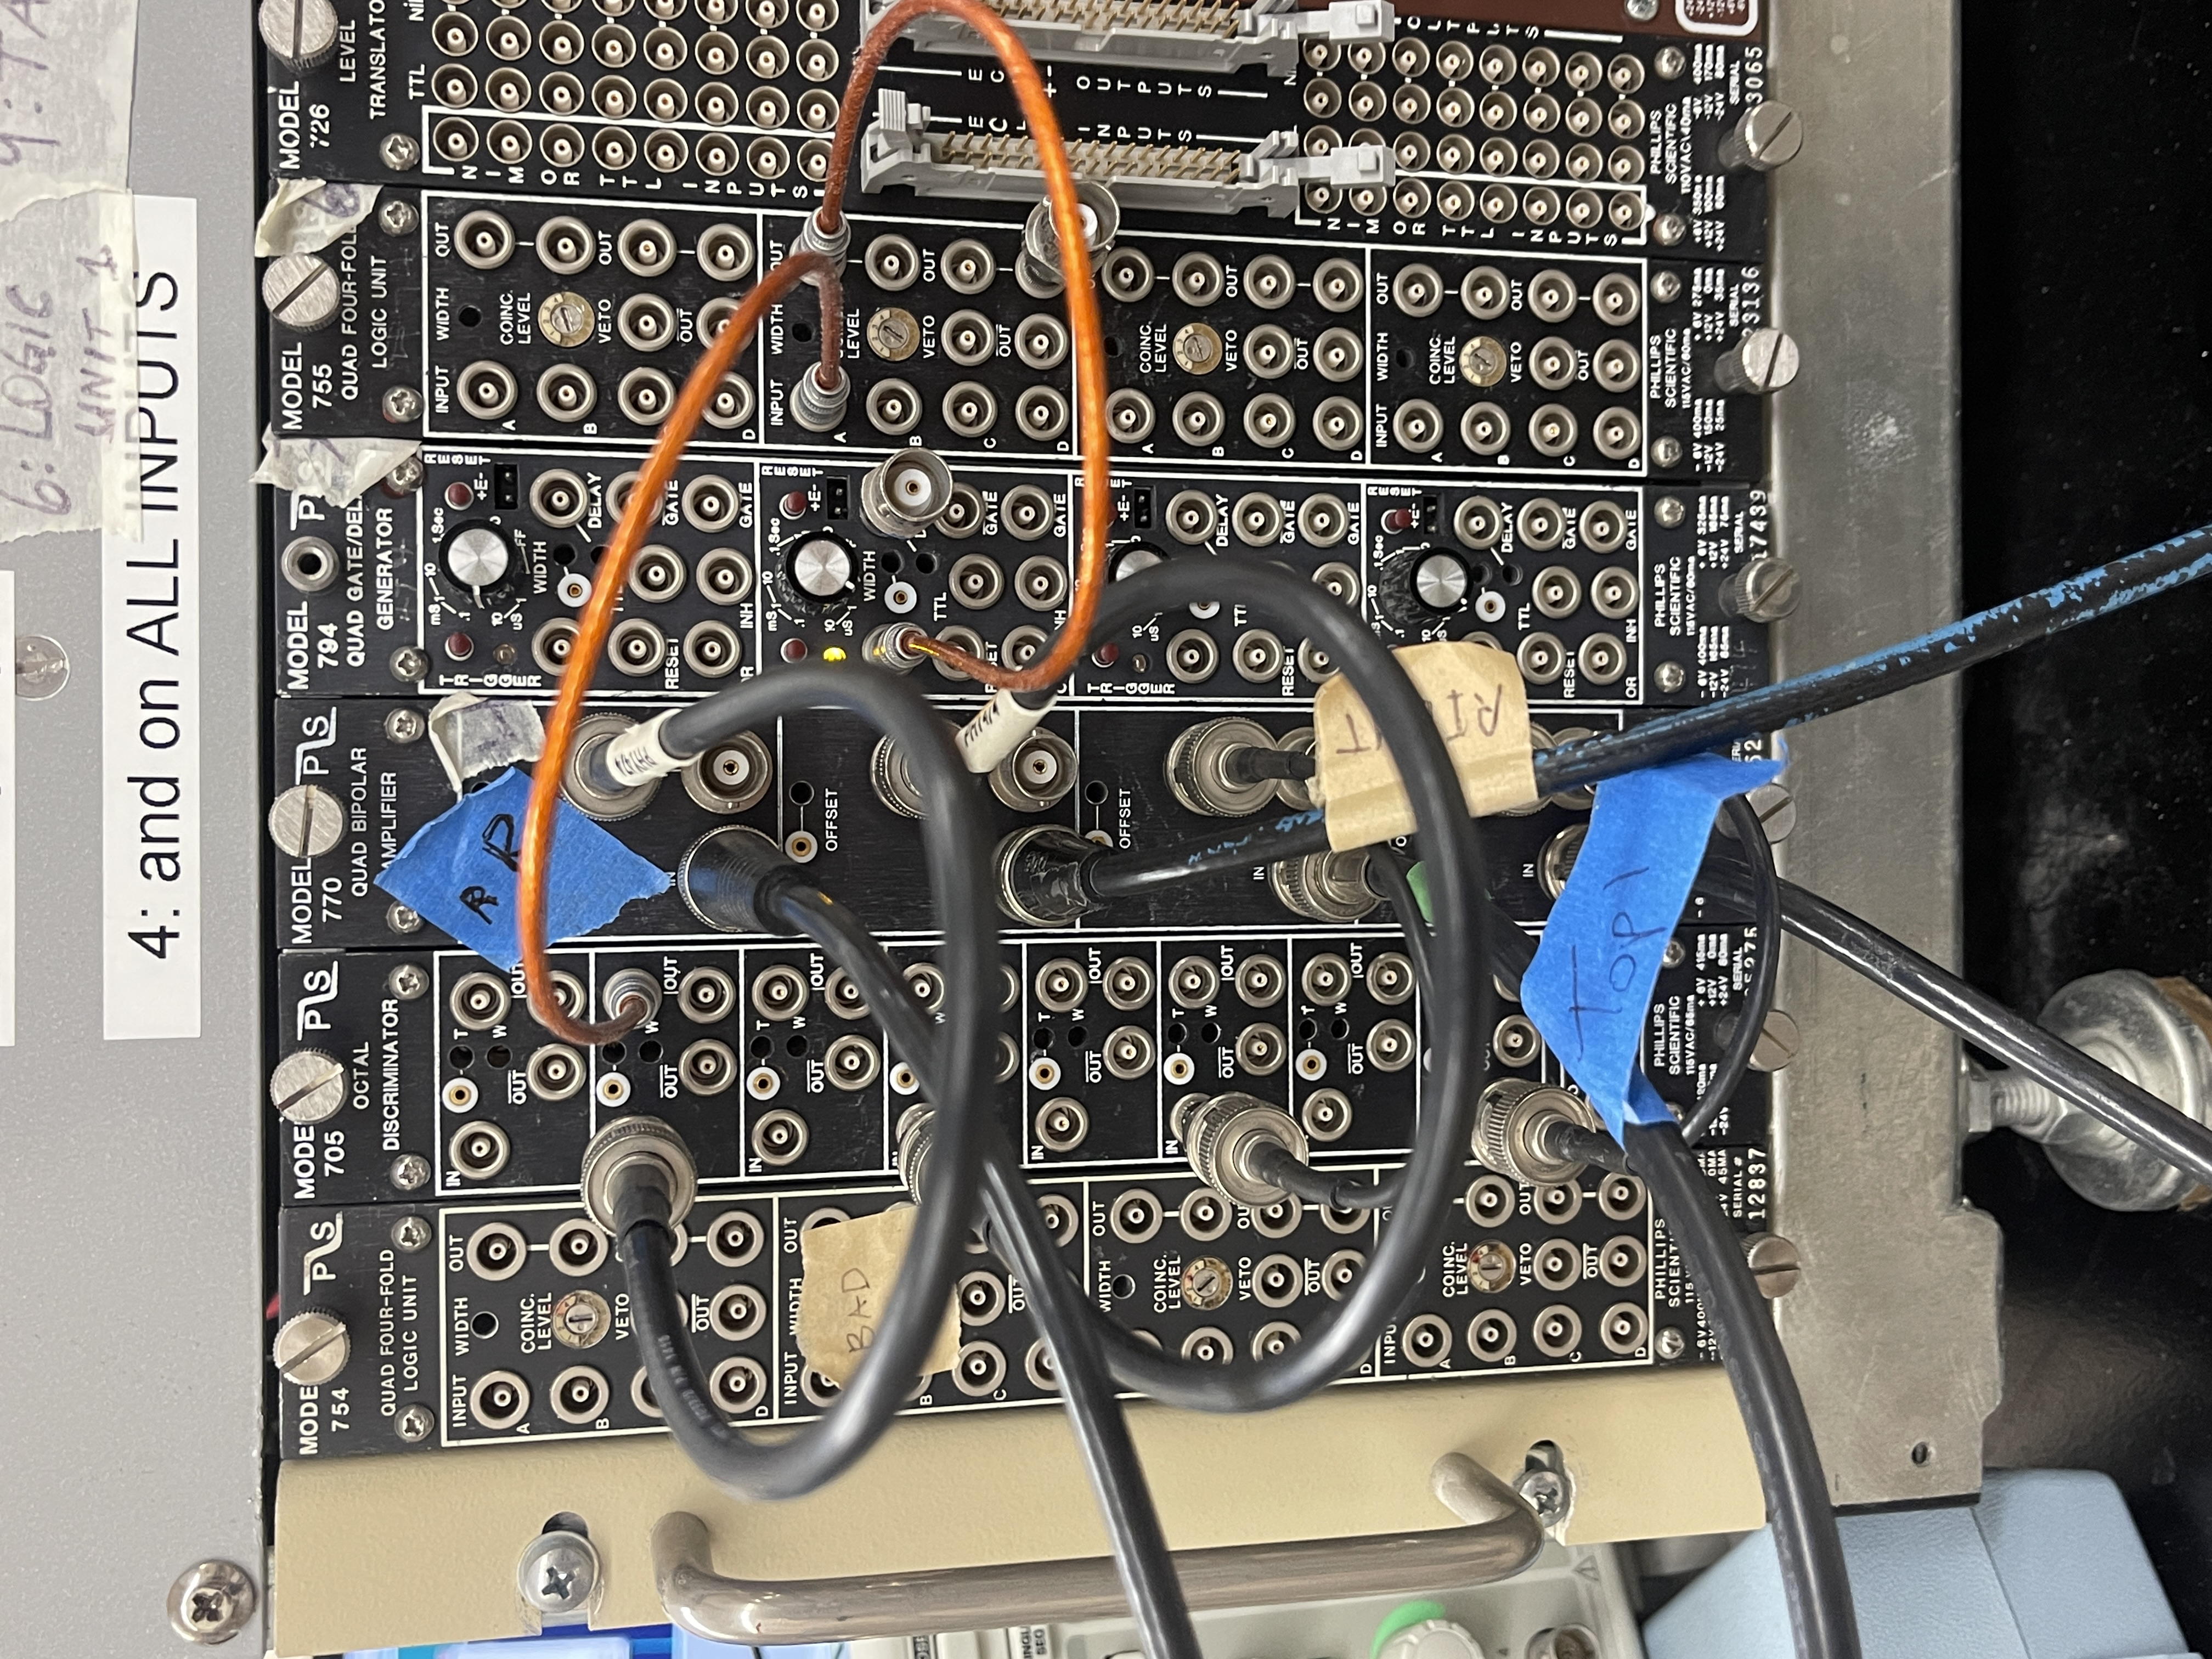
\includegraphics[width=6cm, angle = 270]{Apparatus008.JPG} }}%
        \caption{Here, we have the Philips components, shown on the right. These include the logic component, delay generator and discriminator. On the left, we have our MCA, TAC, and time calibrator, which were manufactured by ORTEC.}%
        \label{fig:apparatus}%
    \end{center}
\end{figure}
\subsubsection{Photomultiplier Tube}

A Photomultiplier Tube (PMT) is a highly sensitive photodetector that is widely utilized in the detection and measurement of low levels of light, ultraviolet (UV), and near-infrared (NIR) radiation. The device operates on the principle of photoelectric effect combined with secondary emission to achieve a high level of signal amplification. A typical PMT consists of a photoemissive material coated cathode, a series of dynodes, and an anode.


The operational mechanism of a PMT begins with the absorption of incident photons by the photoemissive cathode, leading to the emission of photoelectrons due to the photoelectric effect. These photoelectrons are then accelerated towards the first dynode by an electric potential difference. Upon colliding with the dynode, each photoelectron induces the emission of multiple secondary electrons. This process is repeated across a series of dynodes, each at a progressively higher potential, resulting in an exponential increase in the number of electrons. The amplified electron stream finally reaches the anode, producing a measurable current that is proportional to the intensity of the incident light. 

A photo of one our photomultiplier tubes can be found in Figure \ref{fig:rightpmt}. This is the rightmost PMT in our setup.

\begin{figure}[hbt!]
    \begin{center}
        {{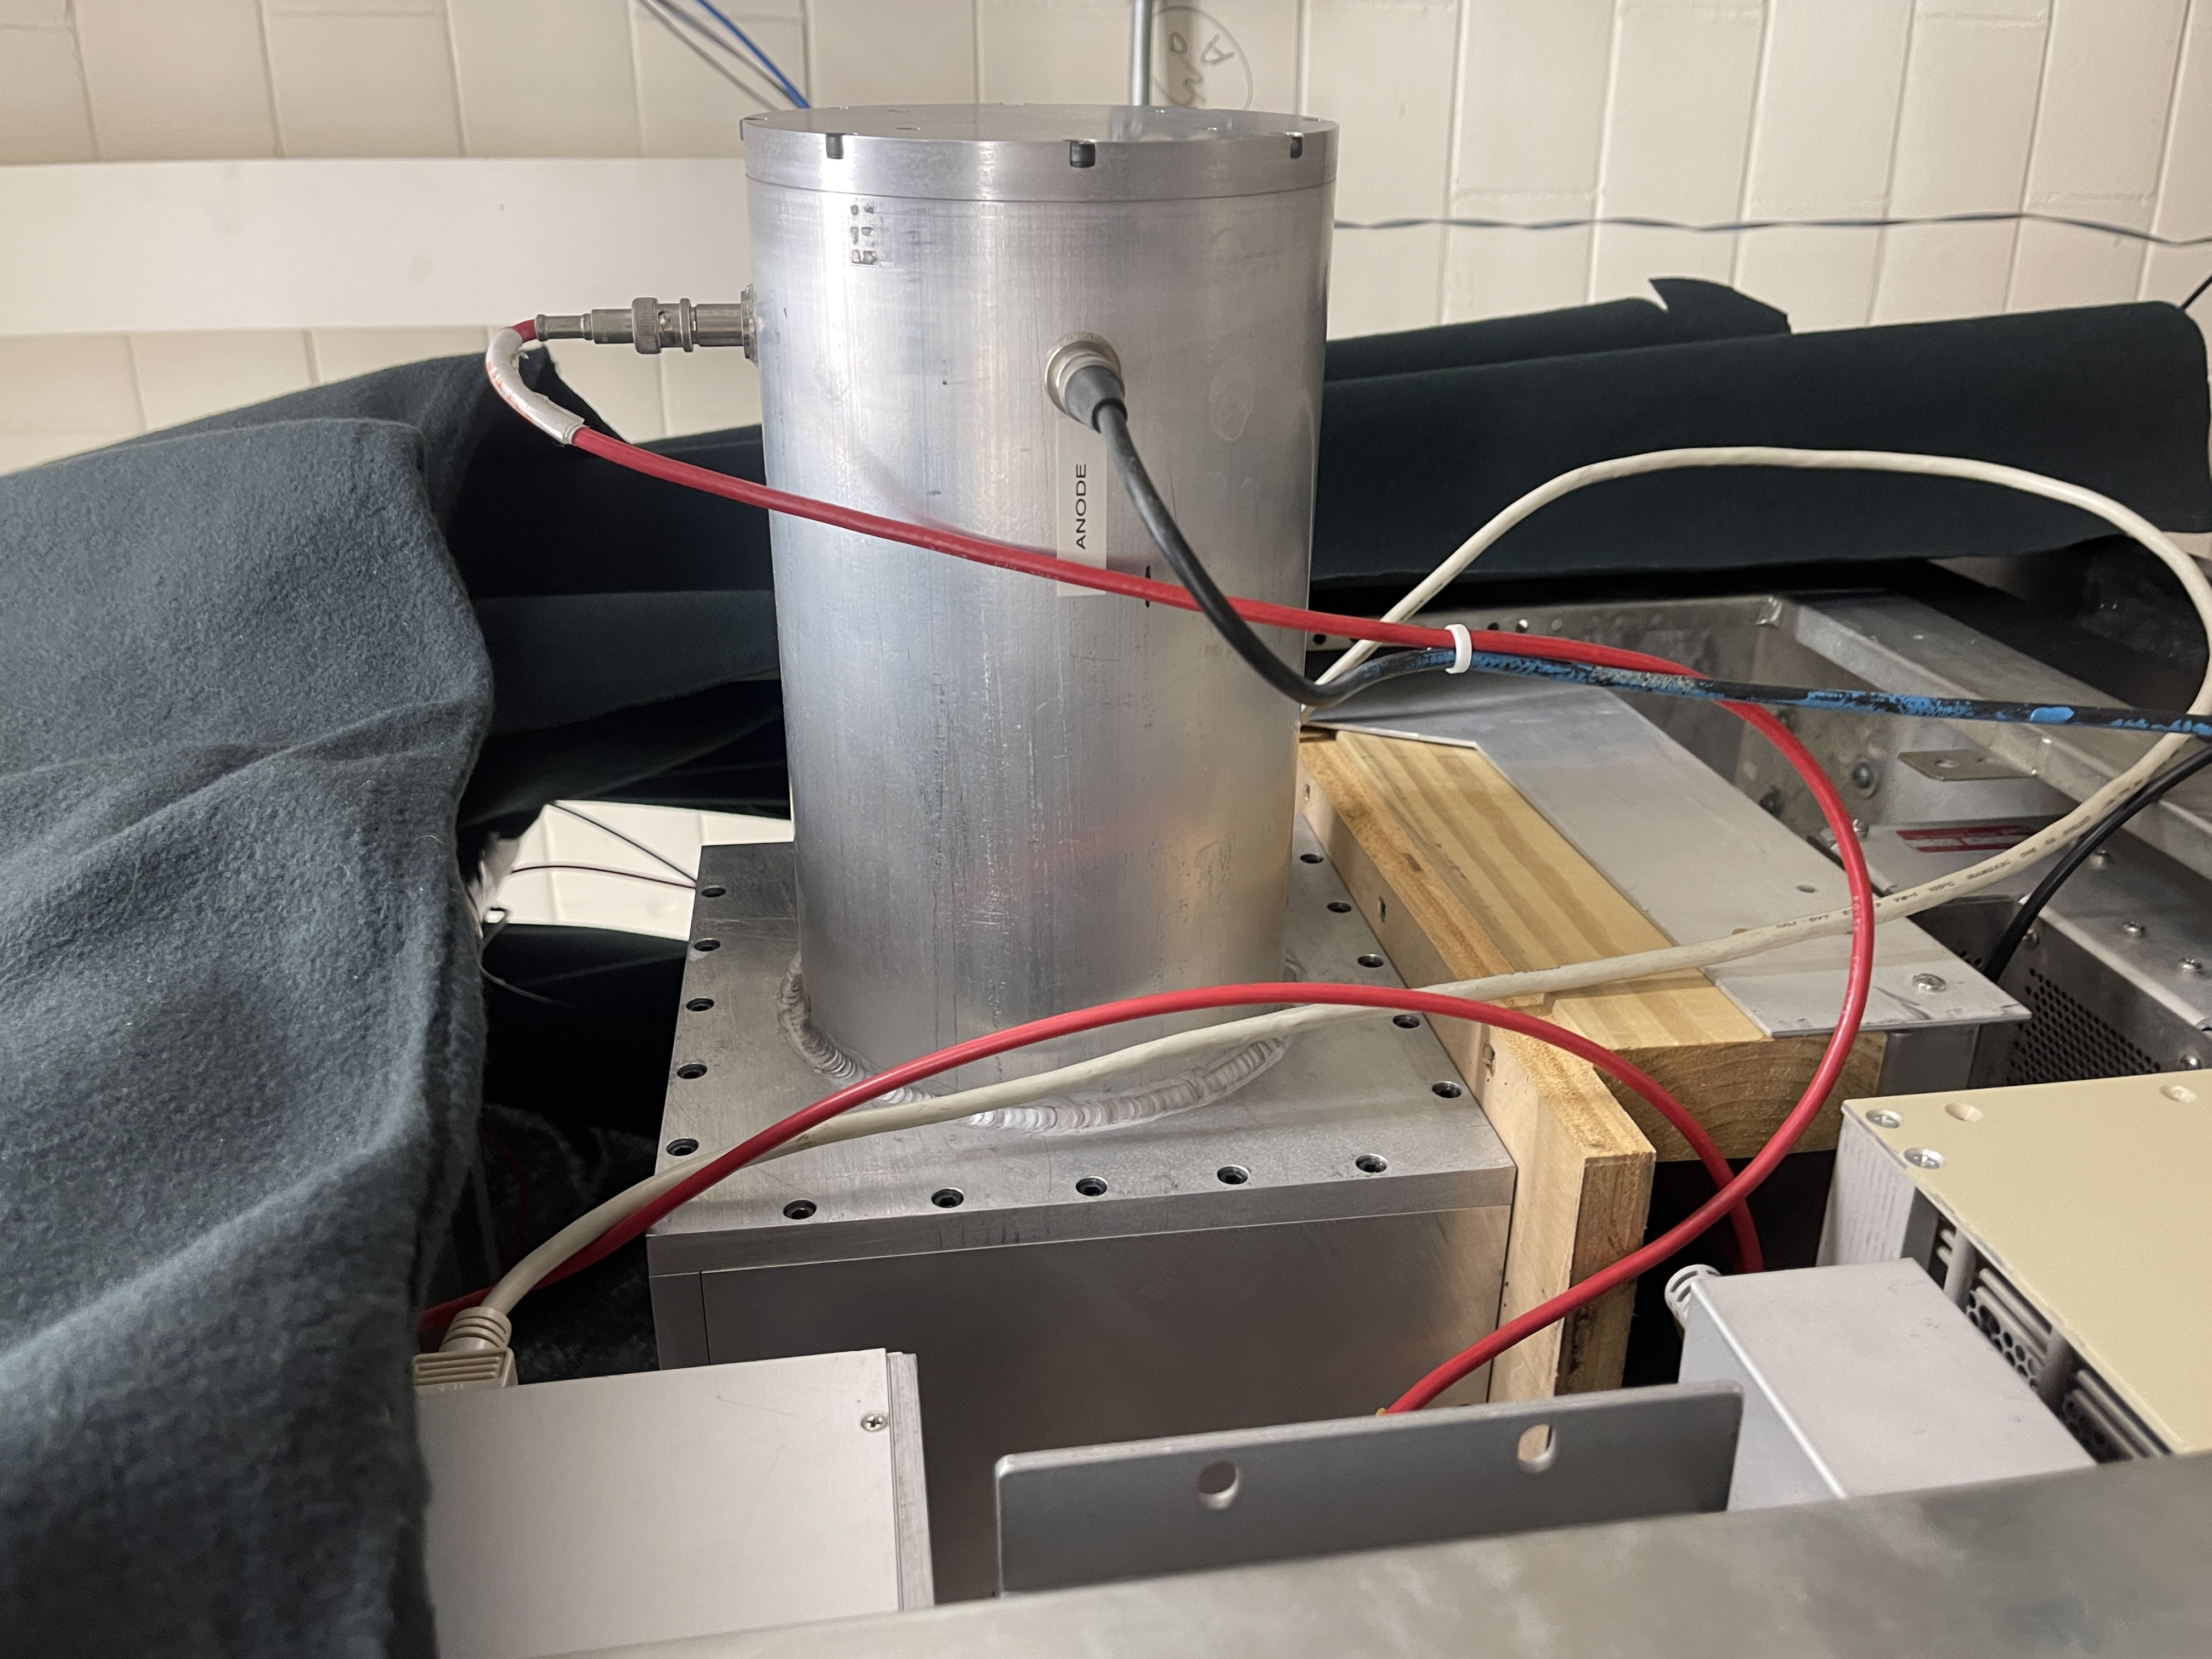
\includegraphics[width=7cm, angle = 270]{Apparatus001.JPG} }}%
        \caption{A picture of our rightmost photomultiplier tube. This tube, and its left counterpart were used to take data, as they are directly attached to the lead glass box.}%
        \label{fig:rightpmt}%
    \end{center}
\end{figure}
\subsubsection{ORTEC and Philips Components}
\begin{figure}[hbt!]
    \begin{center}
        {{\includegraphics[width=8cm]{Apparatus000.JPG} }}%
        \caption{A photo of our high-voltage power supply. Each knob and dial combination directs a voltage to the corresponding PMT or scintillator it is wired to. We set our voltage to 1.3 kV.}%
        \label{fig:psu}%
    \end{center}
\end{figure}
The main ORTEC and Philips Components are the ORTEC 462, 927, and 566, as well as the Philips 705, and 755, as well as a high voltage power supply.

The Philips 705 and 755 are the discriminator unit and the logic unit, respectively. The discriminator allows for the exclusion of false signals from any input, and the logic unit allows us to perform logical operations (such as AND and OR) on our signals.

The ORTEC 462 is a time calibrator, used to calibrate our time measurements. The ORTEC 566 is a time-to-amplitude converter (TAC). This is used to differentiate the time between a start and a stop signal. The output of this TAC is piped into the ORTEC 927, which is our multi-channel analyzer (MCA). The MCA counts are then output to our computer. A loose photo can be seen in Figure \ref{fig:apparatus}
\subsubsection{Computer Software}
To capture the output from the MCA, we use MAESTRO, a software that plots the MCA's counts in a human-readable format. 
\subsection{Data Collection}
Figure \ref{fig:box} depicts our wiring for our components. As our wiring was the same, this figure was taken from Yuchen Gao's report. \cite{gao2018measurement}. To simplify the diagram, the TAC receives a START signal when the muon passes through the topmost PMT. This signal is cancelled out if the bottom PMT is activated within 15 nanoseconds of this signal. This procedure is in place to make sure the muon did not pass through the scintillating box. The TAC also receives its STOP signal when the left OR right PMTs are activated. This stop signal is also vetoed by a top OR bottom signal, as this would indicate perhaps a muon passing through the box at an angle, or not getting fully trapped within the apparatus.

These errors are more clearly described in figure \ref{fig:error}. This figure shows how different muons can pass through the apparatus. The only muons we want to capture and time are muons that follow path 1. 

Typically, a data run would be taken anywhere from 2 to 4 days. This was done to reduce variance and so-called statistical errors that originate from the innate randomness of particle decay.
\begin{figure}[hbt!]
    \begin{center}
        {{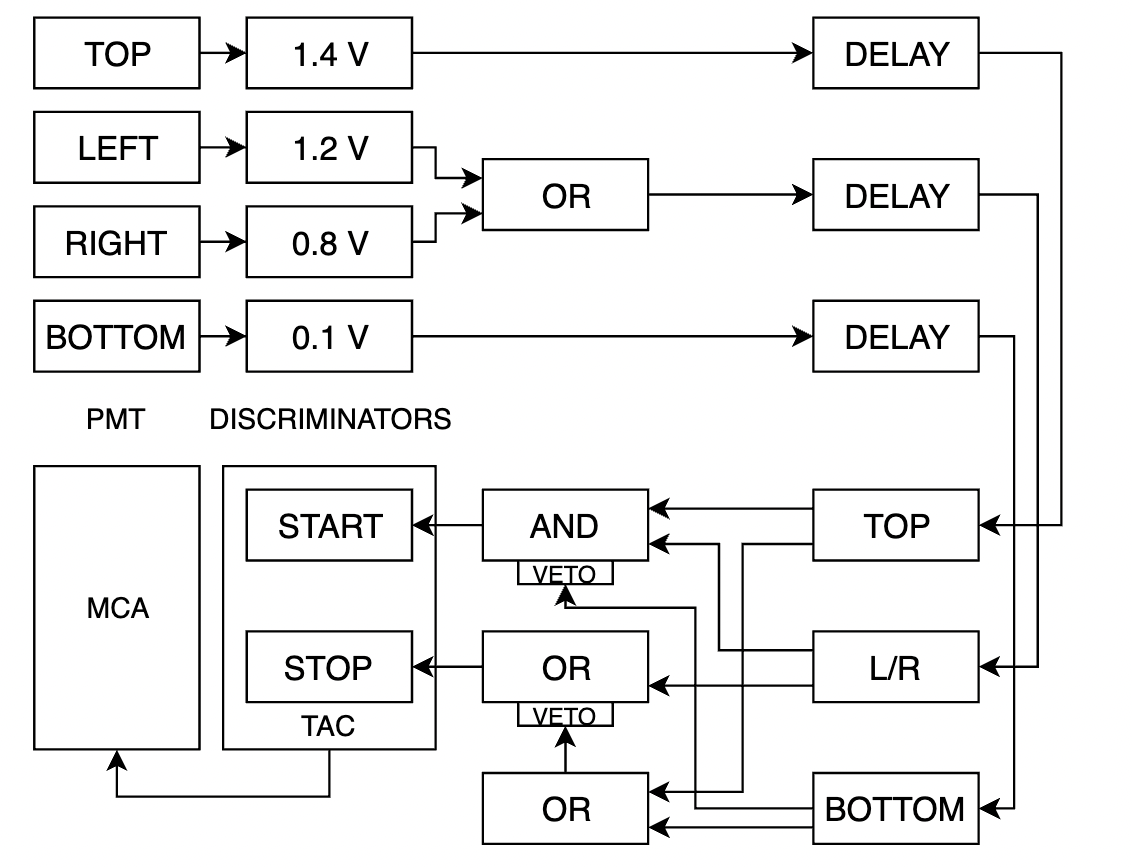
\includegraphics[width=10cm]{BoxDiagram.png} }}%
        \caption{A diagram depicting our wiring for our experiment. This was taken from Yuchen Gao's lab report, written in 2018. \cite{gao2018measurement}.}%
        \label{fig:box}%
    \end{center}
\end{figure}

\begin{figure}[hbt!]
    \begin{center}
        {{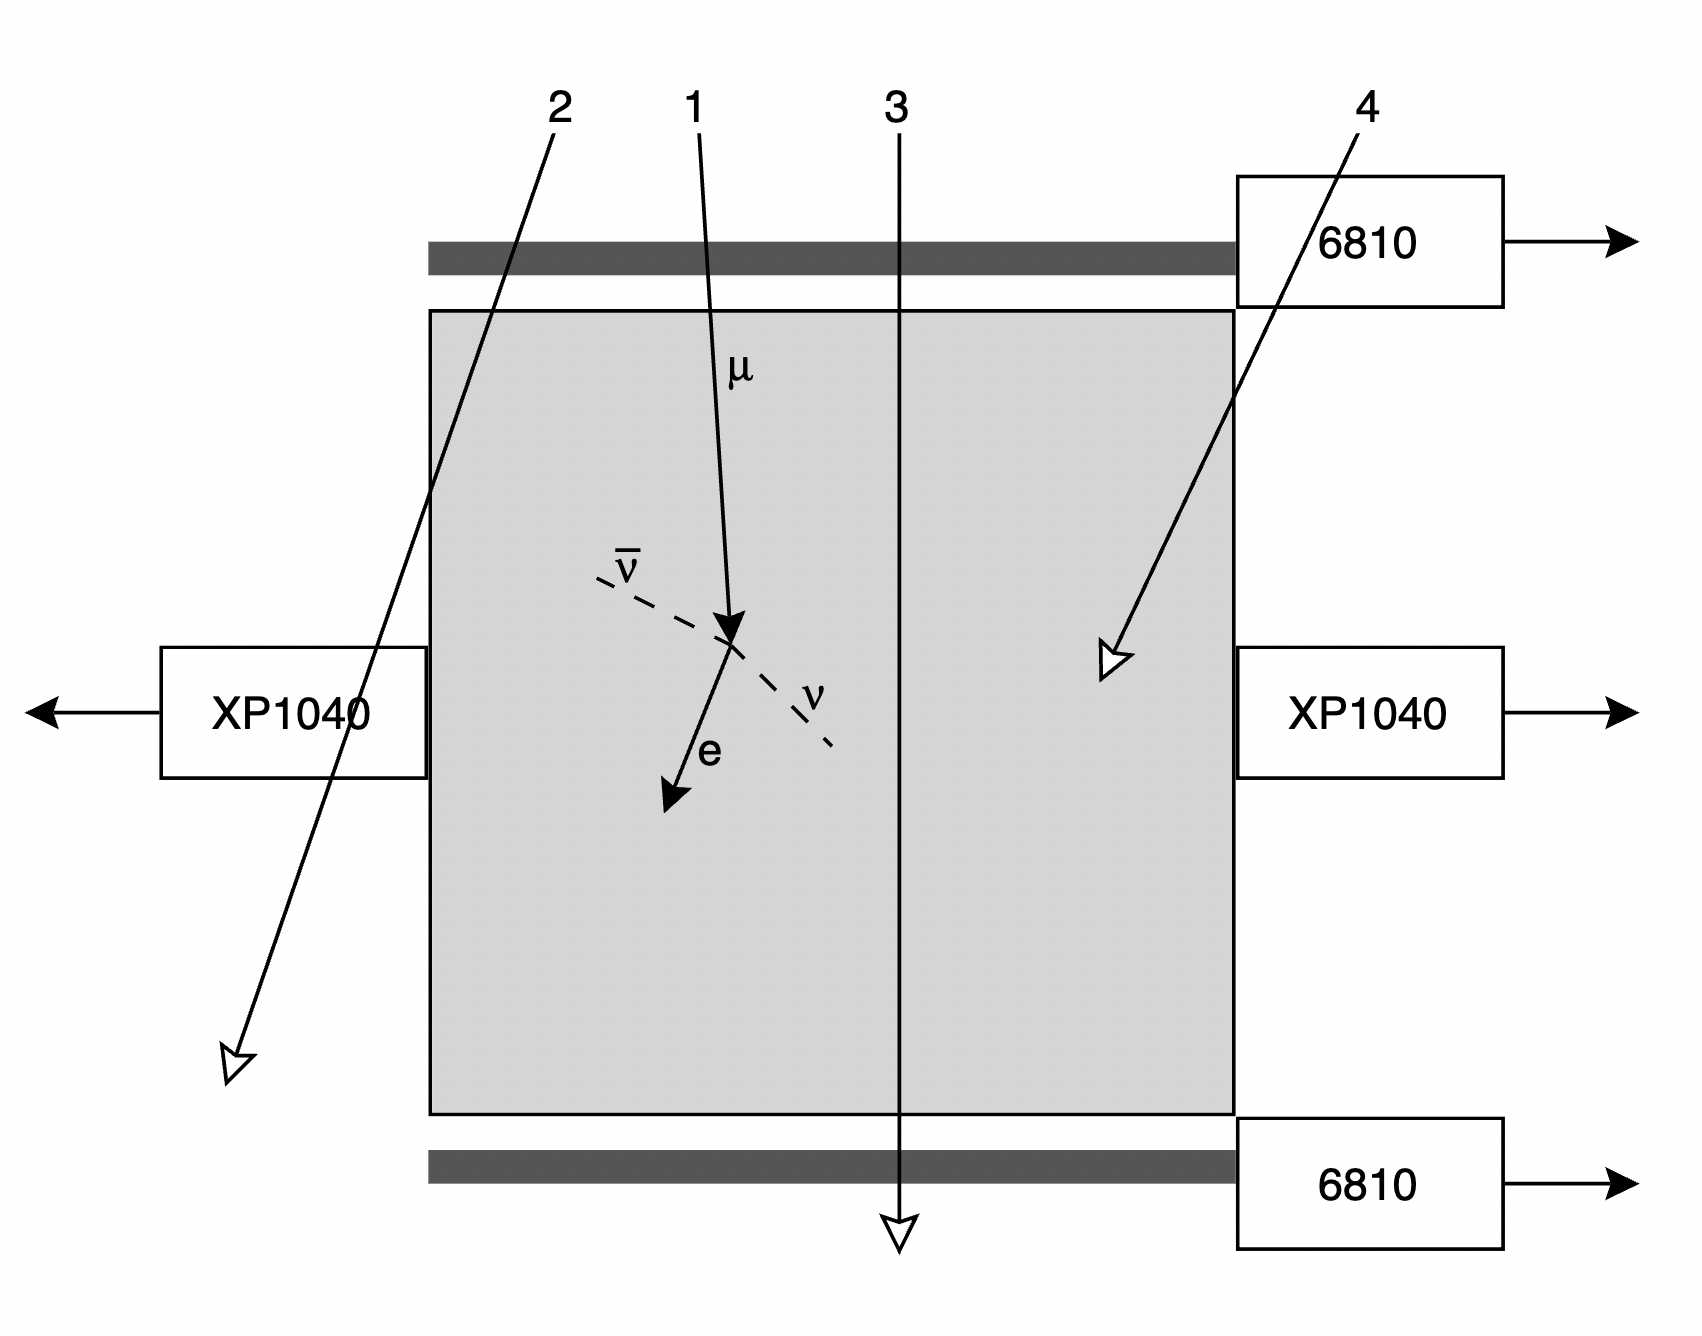
\includegraphics[width=10cm]{errorbox.png} }}%
        \caption{A diagram depicting the path of different muons through our apparatus. Taken from Mike Romalis's lab manual for a similar experiment done at Princeton \cite{princeton}.}%
        \label{fig:error}%
    \end{center}
\end{figure}
\section{Data Analysis}
\subsection{Calibration}
Our calibration method involved setting an ORTEC 462 Time Calibrator to a variety of different times, then running these signals through our TAC. From there, we run our TAC output to our MCA, and we can identify how the MCA's 'bins' correlate to real world times. 

Figure \ref{fig:calib} shows the counts vs. bins data for our calibration setup. Each peak is 640 nanoseconds apart. Furthermore, the height of each peak bears no relevance to our measurements, as it is an arbitrary length of time that the peak was selected for. From this calibratin data, we only analyze how many bins away each peak is from the next. After analysis, we found each peak to be 1066 bins away from the next peak, leaving us with the relation

$$
\text{Time(s)} = 6.01 \times 10 ^ {-4} \times (\text{bin})
$$
\begin{figure}[hbt!]
    \begin{center}
        {{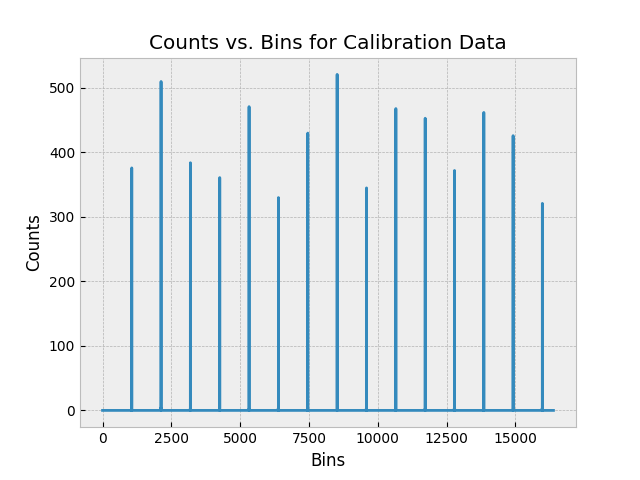
\includegraphics[width=10cm]{calib.png} }}%
        \caption{A figure depicting our counts vs. bins for some of our calibration data. This data was taken with each peak being .64 microseconds apart, for 10 microseconds.}%
        \label{fig:calib}%
    \end{center}
\end{figure}
\subsection{Experimental Data}
Our experimental data came from a run that lasted approximately 52 hours. During this run, we encountered a large number of counts that showed an extremely small time for the muon decay. Many of these counts were omitted from our analysis. Figure \ref{fig:init} depicts the magnitude of these zero bin counts in our data. We decided to analyze data from bin 2500 onwards, as this was the most experimentally exponential data.

After fitting an exponential curve to this data, we were able to determine a mean lifetime of 2.43 $\pm$ .22 microseconds for the particles we observed.

However, our analysis included the use of a Savgol filter, which reduces high frequency noise in a signal. Therefore, our 'real' error may be higher than our calculated one.
\begin{figure}[hbt!]
    \begin{center}
        {{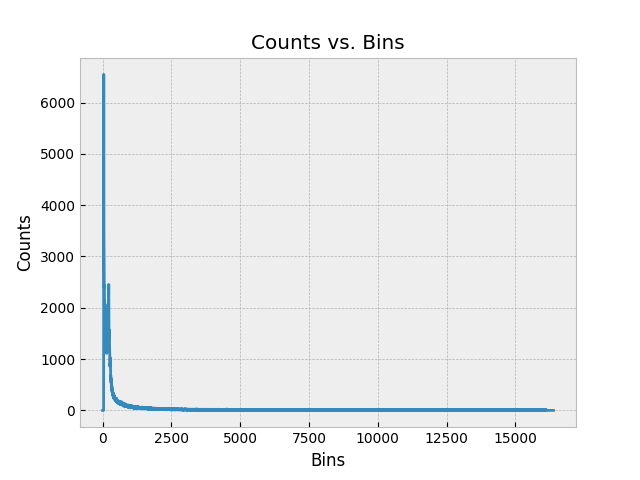
\includegraphics[width=10cm]{initData.png} }}%
        \caption{A figure depicting our raw counts vs. bins for our experimental data. As we can see, the zero counts are on completely different orders of magnitude from the others.}%
        \label{fig:init}%
    \end{center}
\end{figure}
\subsection{Error and Uncertainty}
Much of our anticipated error stemmed from muons escaping the box, or passing through the box at odd angles. Furthermore, we saw thousands of counts that were too low in amplitude to come from muon events. Since these data points were omitted, this may be a point of concern to analyze in the future.
\section{Results and Conclusions}
\subsection{Results}
The experimental data successfully determined the lifetime of the muon within two standard deviations of the accepted value. However, due to the nature of our analysis, this result is accurate, but likely imprecise. We were able to determine the lifetime of the muon to be 2.43 $\pm$ .22 microseconds
\subsection{Conclusion}
In conclusion, we observed muons entering the setup and decaying within it. The goal of this experiment was to observe muons and determine their lifetime, and we have successfully done so.
\paragraph*{Acknowledgments}
I would like to thank my lab partner, Nirmal Patel for his assistance on data collection. Furthermore, I'd like to thank Dr. Deepa Thomas, Matthew Dwyer, and Erick Martinez for their assistance throughout the measurement and set up processes. 

\newpage
\bibliography{refs} 

\end{document}

